\documentclass{article}
\usepackage{graphicx}
\usepackage{indentfirst}
\usepackage{caption}
\usepackage{subcaption}
\usepackage{amsmath}
\begin{document}
  \author{Siqi Wu\\ Tianxiao Zhang \\ Siqi Bian (Susie)\\ Minhao Cheng}
  \section{Introduction}
  \section{Data Collection}
\subsection{Raw Data}
      To collect data from Yikyak, we used a Python program to retrieve yaks from YikYak server. That program could collect yaks of current moment and a specific geographic location. The original version of this program just print out all yaks it retrieved, We slightly changed the program to make it could write the result to a csv file. We set the time interval of collecting data to one hour, since normally the oldest yaks it could get is one to two hours ago. We collected around 24000 yaks at the end.
    \subsection{Data Processing}
      Because of the one-hour interval, there is some duplicate yaks, the first thing we should do is to get rid of these duplicate yaks. Besides, there are also some unnecessary information like number of like, user id and time, we also need to delete that part. Finally, what left is only the text.

      Another challenging problem is to processing the emoji, I planed to replace them with plain text, like should be replaced by $Emoji(Smiling_Face)$, thus we could treat an single emoji as a single word, which is very reasonable. After tackling several encoding and decoding problem, I finally replaced all emojis with plain text, which is the description of that emoji.

    \subsection{Labeling Data}
      Since we are doing supervised learning, we need all data labeled. There is not better way than label by human being, actually that might be the only way to label the data. In that sense, the Mechanical Turk is a good choice for us, we upload about 6000 yaks to Mechanical Turk and let workers to work on it. In order to get a relatively accurate label, each yak is labeled by 5 people, and according to their answer, we average them to get a final label.

      After all these processing and labeling procures, we have around 6000 labeled data.

  \section{Lexicon Classifier}
    Lexicon Classifier is probably simplest sentimental classifier, what we need is just two dictionaries, one for positive words while another is for negative words. There is no training process in lexicon classification, we only need to compute the number of positive words $p$ in a text, and negative words $n$. If $p>n$, we assign this text with "positive", otherwise, if $n>p$, the text is "negative".

    This most straightforward method could intuitively give us a label of one text, the accuracy of the method is 52.3\%.
  \section{Na\"ive Bayes}
    \subsection{Bayes' Theorem}
      By first observing that by Bayes' rule,
      $$P(c|d)=\frac{P(c)P(d|c)}{P(d)}$$,
      where $d$ stands for document, in our situation, yaks, while $c$ indicates class. Then, we could compute the class membership probabilities of each class,
      $$P(c_j|d)=\frac{P(c_j)\prod_i P(w_i|c_j)}{P(d)}$$,
      where $w_i$ are words in $d$, and the class which has highest probability will be predicted.

    \subsection{Implementation}
      In practical, we want to classify one text into three class: Positive, Negative, Neutral. So we transfer this multi-class problem to a binary-class classification problem, i.e. we train two different classifiers, one is positive v.s. non-positive while other one is negative v.s. non-negative. 

      Then, according to the formula, we calculate the priori probabilities using training data. When predict a certain text, we use the pre-computed probabilities to calculate each class' probabilities and then predict the final label. One potential problem is that what if a word is not included in training set? Here we introduce add-one-smooth to solve this problem, i.e. calculate the conditional probability as follow:
      $$P(w_i|c_j) = \frac{count(w_i,c_j)+1}{count(w,c_j)+|V|}$$.

    \subsection{Result} 
      Accuracy of Na\"ive Bayes is 56.9\%.
  \section{Feature Selection}
  \subsection{Theorem}
  A major problem appears in dealing with text. The text is in very high dimensionality of the feature space. It could make the supervised training model like neural network hard to work. On the other hand, due to the independence assumption in the Naive Bayes method, supervised learning method like SVM achieve the best performance so far. Therefore, we want to reduce the dimension of feature to make our training more efficiently and reliably. So feature selection is a popular method in natural language processing.\\
  There are a lot of method in feature selection. In our work, we choose five feature selection method as follows to test our data.
  \subsubsection{Information Gain}
  Information gain is the fundamental theorem in machine learning method like decision tree. It measures the number of bits of information obtained for category prediction by knowing the present or absence of the item. In our case, it is the information we achieve from each word in the feature space. Let $c_i$ denote the class type in the space. The information gain of item t is defined like this:
  \begin{equation}
  \begin{split}
  G(t)&=Pr(t)\sum_{i=1}^{m}Pr(c_i|t)logPr(c_i|t)+Pr(\bar{t})\sum_{i=1}^{m}Pr(c_i|\bar{t})logPr(c_i|\bar{t})\\
  &-\sum_{i=1}^{m}Pr(c_i)logPr(c_i)
  \end{split}
  \end{equation}
  In our work, there are 3 types of class: negative, neutral, positive. They are represented by $c_1,c_2,c_3$ respectively. t is each word, $\bar{t}$ is that t doesn't show up. After getting all the information gain, we will set a threshold to do the feature selection word. We remove those words whose information gain are below the threshold, which means we can not get enough information from this word. However, how to set the threshold is very tricky. Since there are a lot variety in our data, a little change in threshold will make the performance drop from good to very bad or just rise a little bit.
  \subsubsection{Document Frequency Thresholding}
	Document frequency is the number of documents in which a term occurs. It is simplest way of feature selection. We compute the frequency of each word in our datasets. Again, we remove those whose frequency are below certain threshold.\\
	However, in our case, because of the user's diversity, their words are almost different from others. If you choose this method to do the feature selection, what you got is just the stop words like "a","some","any","but","and" etc. Obviously, the performance will be very bad.
  \subsubsection{Mutual Information}
    The Mutual information is defined as follows:
  \begin{equation}
  I(t,c)=log\frac{Pr(t\land c)}{Pr(t)\times Pr(c)}
  \end{equation}
  We can use 
  \begin{equation}
  I(t,c)\approx log\frac{A\times N}{(A+C)\times(A+B)}
  \end{equation}
  to approximate. Where t is the word, c is the class, A is the number of times t and c co-occur, B si the number of time the t occurs without c, C is the number of times c occurs without t, and N is the total number of our samples. The advantage of mutual information is that the it is strongly influenced by marginal probabilities of terms. It looks very suitable for our case.[6]
  \subsubsection{Other Method}
  There are other methods like $\chi^2$ statistic, term strength etc. They are all used wildly in statistical language modeling of word associations and related applications[5].\\ $\chi^2$ statistic is very similar to mutual information method. The difference of $\chi^2$ statistic is that it is a normalized value. However, this normalization breaks down when the term is lightly weighted. Hence it is not good for low-frequency terms. Term strength is originally proposed and evaluated by Wibur and Sirotkin for vocabulary reduction in text retrieval, and later applied to text categorization. The basic idea is estimate term importance based on how commonly a term is likely to appear in "closely-related" documents.
  \subsection{Procedures}
  In our algorithms, we must get every word's information gain to finish the remove procedure. So first, we derive all the words in our datasets. We look into each word's case. When it appears in the sentence, derive the probabilities of negative, neutral, positive sentences respectively. On the other hand, derive the probabilities of negative, neutral, positive sentences respectively when the word is not appears. There is some trick that we can recorded the word we have tested so that we can just omit same word after, which can save a lot of time complexity. Then we calculate the ration of negative, neutral, positive sentences respectively. After we get all terms probability, we just use the equation in information section to get the information gain.
  \subsection{Result}
  Just take a simple example, in our datasets, there is a sentence like this: "Any girls want to relieve some stress rn?". We can get the information gain of each word in this sentence: 
  [0.21115577032085886, 0.21425361540178134, 0.20656925945026372, 0.14608334896615238, 0.22054756983147317, 0.21354746233433897, 0.22270583193338855, 0.22057868402948322].
  If we set the threshold $\theta=0.17$, the word t will be removed. And the sentence will become "Any girls want relieve some stress rn?". It is quite straight-forward. \\ 
     However, how to set the threshold is very tricky. The threshold is depended on the training data. Therefore, a good method is to plot a picture which shows the relation between threshold and accuracy. In our Yik Yak dataset, the error rate looks like this:
     \begin{figure}
     \centering
     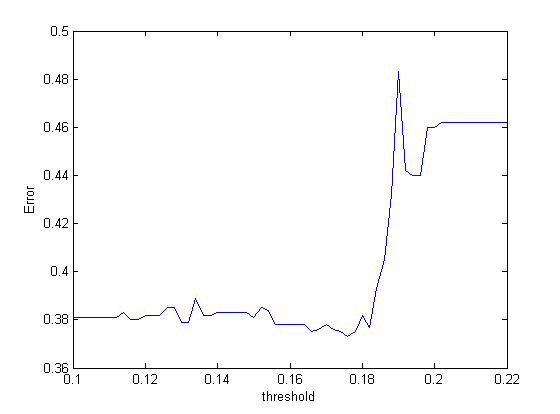
\includegraphics[width=1\textwidth]{evt.png}
     \caption{Error vs Threshold in Yik Yak Data}
     \end{figure}
     As showed, we can see in about 0.175,the error rate is minimal. However, in our twitter dataset, the error rate is like this
          \begin{figure}
          \centering
          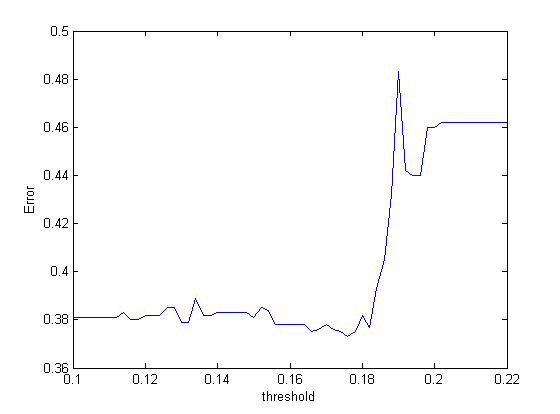
\includegraphics[width=1\textwidth]{evt.png}
           \caption{Error vs Threshold in Twitter Data}
          \end{figure}
  \section{Support Vector Machines}
    Support Vector Machines (SVMs) is a set of good supervised learning methods and we used it as our second sentimental classifier on our yak data because there are lots of advantages of this method such as effective in high dimensional spaces, memory efficient, and so on. 
    \subsection{Theorem}
      Given training vectors $X_i$, $(i = 1,?,n)$, and the class vectors $y \in {1,-1}^n$.  Here is the primal function of the SVM
      $$min_{\omega,b,\zeta}\frac{1}{2}\omega^T\omega + C\sum_{i=1}\zeta_i$$ 
      subject to $$y_i(\omega^T\phi(x_i)+b)\geq 1-\zeta_i$$, $$\zeta_i \geq 0, i = 1,...,n$$
      The corresponding dual function is 
      $$min_{\alpha}\frac{1}{2}\alpha^TQ\alpha - e^T\alpha$$ subject to 
      $$y^T\alpha = 0, 0 \leq \alpha_i \leq C, i = 1, ..,n$$
      where e is the vector of all one, $C > 0$ is the upper bound. $Q_{ij} = y_i y_j K(x_i, x_j)$ where $K(x_i, x_j)$ is the kernel function. We chose to use linear kernel because of the less time spending and good results providing. Thus, $K(x_i, x_j) = <x,x?>$. The decision function is 
      $$sgn(\sum_{i=1}y_i\alpha_iK(x_i,x) + \rho)$$

    \subsection{Procedures}
      It is necessary to preprocess the text documents for applying the SVM method on them, such as turning them to the feature vectors. 
      First, we convert the collection of the texts to a matrix of words count with removing the English stop-words. However, there will be some discrepancies showing up between longer documents and shorter ones which talking about the similar topics. Thus, a method called Term Frequency times Inverse Document Frequency (tf-idf) should be applied here. This method aims to avoid the potential discrepancies by two procedures. The first one is to divide the occurrence number of each word in a yak by the total number of words in the yak. The second one is to downscale the weights for words that show in many yaks through the whole dataset because this kind of words are usually less informative than those with less showing times. For example, think about the word ?am?. It shows commonly in yaks but won't tell us useful information. After finishing the above preparation procedures, we start to build our SVM model.


    \subsection{Results}

      As for the training data split, first we split the data as positive, non-positive, negative and nonnegative, same with the Na\"ive Bayes method, then we got the accuracy score 61.9\%. After that, we split the data as positive, neutral and negative directly and apply the model. Then we obtained a higher accuracy score 63.5\%. 

    \subsection{Compare with the twitter}  
      We used the twitter dataset, which have the same train and test data size and structure with the yak dataset. Apply the same model and then we obtained the accuracy score 61.5\% if splitting as positive, non-positive, negative and nonnegative, and 64.6\% if splitting as positive, neutral and negative directly.
  \section{Reference}
  Text Categorization with Support Vector Machines: Learning with Many Relevant Features 
  Thorsten Joachims
  [5]R.Fano Transmission of information. MIT Press, Cambridge, MA, 1961
  [6] T.E. Dunning. Accurate methods for the statistics of surprise and coincidence. In Computational Linguistics, volume 19:1, pages 61-74, 1993
  
\end{document}